\chapter{计算机网络和因特网}

\section{什么是因特网}

    我们可以用两种方式来回答:

\begin{itemize}
    \item [1)] 描述因特网的具体构成,即构成因特网的基本硬件和软件组件
    \item [2)] 根据为分布式应用提供服务的联网基础设施来描述因特网
\end{itemize}

\subsection{具体构成描述}

    用因特网术语来说,所有这些设备都称为主机($host$)或端系统($end system$)。端系统通过通信链路($comminication link$)和分组交换机($packet witch$)连接到一起。

    通信链路,简单来说就是不同类型的物理媒介,例如光纤,铜线等,而链路的传输速率($transmission rate$)以比特/秒($bit/s$,或$bps$)度量。\emph{当一台端系统要向另一台端系统发送数据时,发送端需要将数据进行分段,然后将每段数据加上首部字节}(很显然,这部分的知识点一开始难以理解,因为是属于更下层的知识)。因此,这样形成的信息包在计算机网络中被称为分组($packet$)。

    而分组交换机就和其名字一样,它接受到达的分组,然后从一条出通信链路转发该分组。目前,最为常见的分组交换机为:路由器($route$)和链路层交换机($link-layer switch$)。

\begin{itemize}
    \item 路由器通常用于网络核心
    \item 链路层交换机通常接入网中
\end{itemize}

    \emph{从发送端系统到接收端系统,一个分组所经历的一系列通信链路和分组交换机}称为通过该网络的路径($orute$或$path$)

    端系统通过因特网提供商($Internet Service Porvider, IPS$)接入因特网,每个\emph{IPS}自身就是一个由多台分组交换机和多段通信链路组成的网络。

\begin{itemize}
    \item 各IPS为端系统提供了各种不同类型的网络接入,同时IPS也为内容提供者提供因特网接入服务
    \item 较低层的IPS通过国家、国际的较高层IPS互联
    \item 较高层的IPS通过高速光纤链路互联的高速路由器组成
\end{itemize}

\subsection{服务描述}

    前面我们辨识了构成因特网的许多部件,此处我们可以从一个完全不用的角度,即\emph{为应用程序提供服务的基础设施}的角度来描述因特网。因为被描述的应用程序涉及多个互相交换数据的端系统,故它们被称为分布式应用程序($distributed application$)。

    需要注意的是:\emph{因特网应用程序运行在端系统上,即它们并不运行在网络核心中的分组交换机中。尽管- 分组交换机能够加速端系统之间的数据交换,但它们并不在意作为数据的源或宿的应用程序。}

    为了使得运行在端上的应用程序能够向另一个端上发送信息,因此就有了套接字接口($socket interface$),该接口\emph{规定了运行在一个端系统上的程序请求因特网基础设施向运行在另一个端系统上的特定目的地程序交付数据的方式}。因特网套接字接口是一套发送程序必须遵循的规则集合。

\subsection{什么是协议}

    理解计算机网络协议($protocol$)最简单的方式显然是用人类本身来类比,因为实际上,我们人类无时无刻不在执行协议。

\begin{figure}[!htbp]
    \centering
    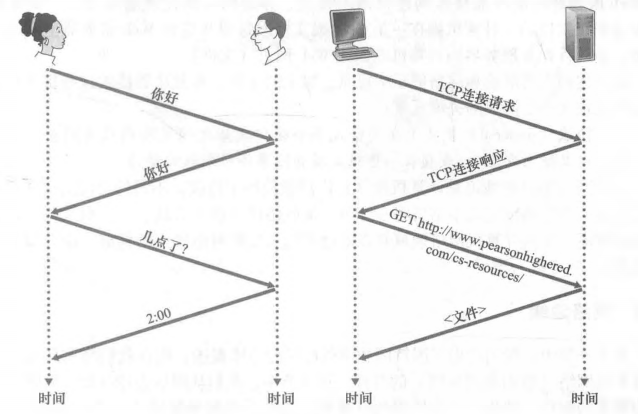
\includegraphics[width=0.6\textwidth]{image/chapter01/人类活动类比协议.png}
    \caption{人类活动类比协议}
\end{figure}

    可以看见,人类协议(或者说好的行为方式)要求一方先发起问候,然后开始与另外一人的通信。那么在计算机中对应的便是,端系统对另一个端系统发起通信。注意:\emph{在我们人类协议中,有我们发送的特定报文,也有我们根据接收到的应答报文或其他事件(例如在某个给定的时间内没有回答采取的动作}。

    那么反过来,如果是一个坏的行为方式(比如一上来就有人破口大骂),那么你也就不想继续进行通信,也就是说,该协议就不能交互,从而无法完成工作。那么网络也是同理。

    网络协议类似于人类协议,在因特网中,涉及两个或多个远程通信实体的所有活动都受协议的制约:

\begin{itemize}
    \item [1)] 硬件实现的协议控制了两块网络接口卡间的“线上”的比特流
    \item [2)] 拥塞控制协议控制了在发送方和接收方之间传输的分组发送的速率
    \item [3)] 路由器中的协议决定了分组从源到目的地的路径
    \item [n)] ...
\end{itemize}

    最终,我们可以得出协议的定义:\emph{协议(protocol)定义了在两个或多个通信实体之间交换的报文的格式和顺序,以及报文发送和/或接收一条报文或其他事件所采取的动作。}

\section{网络边缘}

    在计算机网络中,通常把与因特网相连的计算机和其他设备称为端系统,因为它们位于因特网的边缘。

\begin{figure}[!htbp]
    \centering
    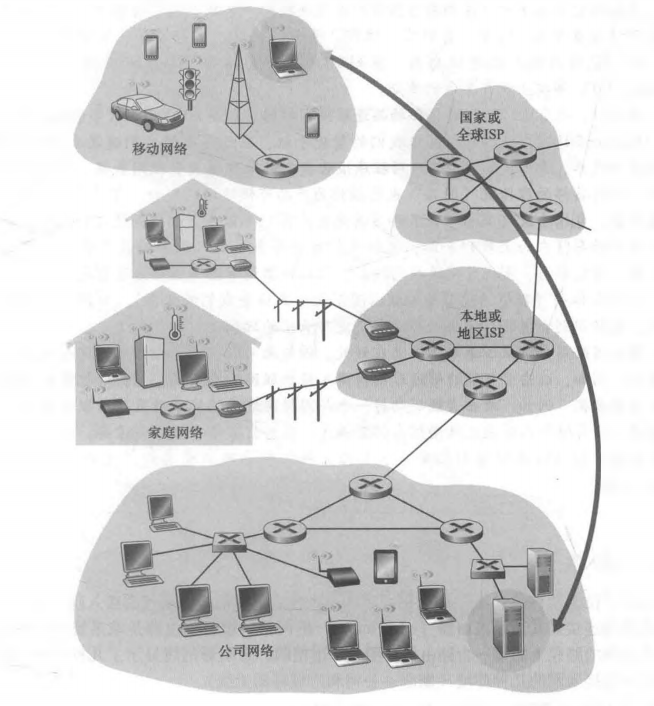
\includegraphics[width=0.6\textwidth]{image/chapter01/网络边缘.png}
    \caption{端系统交互}
\end{figure}

\subsection{接入网}

    接入网是指将端系统物理连接到其边缘路由器($edge router$)的网络。边缘路由器是端系统到任何其他远程端系统的路径上的\emph{第一台路由器}。

\subsubsection{家庭接入:DSL、电缆、FTTH、拨号和卫星}

    如今,宽带入宅接入有两种最为流行的方式:数字用户线($Digital Subscriber Line, DSL$)和电缆。
    
    用户从运营商公司获取DLS接入,通过DLS调制解调器使用电话线与运营商的本地中心局($CO$)中的数字用户接入复用器($DSLAM$)交换数据。用户的DSL调制解调器获得数字数据后将其转换为高频音,通过电话线传输给本地中心局。

\begin{figure}[!htbp]
    \centering
    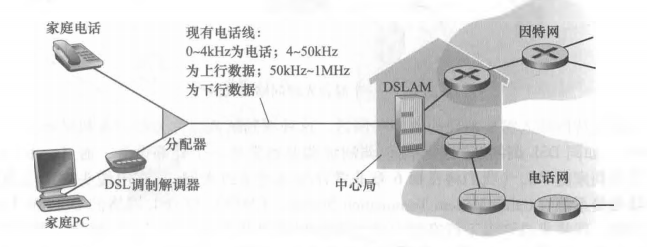
\includegraphics[width=0.6\textwidth]{image/chapter01/DLS接入.png}
    \caption{DSL因特网接入}
\end{figure}

    家庭电话线同时承载了数据和传统的电话信号,且用不同的频率进行编码。这种方法使得一根DSL线路能够看上去像三根独立的线路一样。:

\begin{itemize}
    \item 高速下行信道,位于50kHz到1MHz频段
    \item 中速上行信道,位于4kHz到50kHz频段
    \item 普通的双向电话信道,位于0到4kHz频段
\end{itemize}

    DSL利用了电话公司现有的本地电话基础设施,而电缆因特网接入($cable Internet access$)利用了有线电视公司现有的有线电视基础设施。如下图所示,光缆将电缆头端连接到地区枢纽,从这里使用传统的同轴电缆达到各家各户。因为在这个系统中应用了光纤和同轴电缆,因此被称为混合光纤同轴($Hybrid Fiber Coax, HFC$)系统。

\begin{figure}[!htbp]
    \centering
    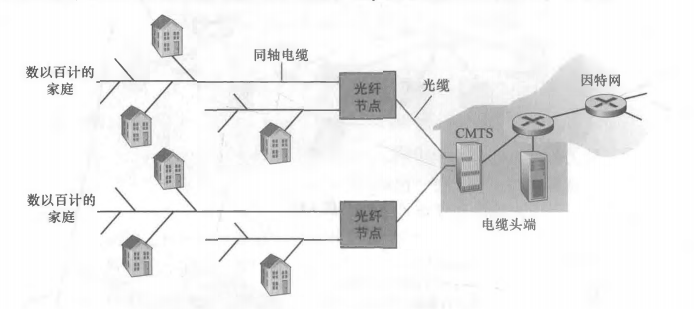
\includegraphics[width=0.6\textwidth]{image/chapter01/电缆接入.png}
    \caption{混合光纤同轴接入网}
\end{figure}

    电缆因特网接入需要特殊的电缆调制解调器($cable modem$)。电缆调制解调器通常是一个外部设备,通过一个以太网端口连接到家庭PC。在电缆头端,电缆调制解调器端接系统($CMTS$)与DSL网络的DSLAM具有类似的功能。

    电缆因特网接入的一个重要特征是\emph{共享广播媒体}。特别是,由头端发送的每个分组向下行经每段链路到每个家庭;每个家庭发送的每个分组经上行信道向头端传输。这就是为什么我们在宿舍高峰期会感觉明显的网速变慢的原因。

    另一种提供更为高速率的新兴技术是光纤到户($Fiber To The Home, FTTH$),顾名思义,FTTH直接从本地中心局到家庭提供了一条光纤路径。

\subsubsection{企业(和家庭)接入:以太网和WiFi}

    在公司和大学校园以及越来越多的家庭环境中,使用局域网(LAN)将端系统连接到边缘路由器。尽管有许多不同类型的局域网技术,但是以太网到目前为止是公司、大学和家庭网络中最为流行的接入技术。

\begin{figure}[!htbp]
    \centering
    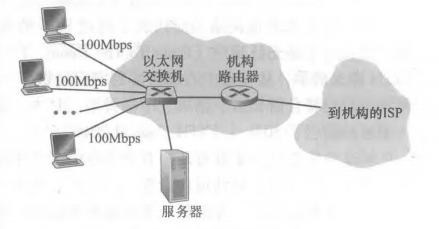
\includegraphics[width=0.6\textwidth]{image/chapter01/以太网接入.png}
    \caption{以太网因特网接入}
\end{figure}

    然而,越来越多的人从便携机、智能手机、平板电脑和其他物品无线接入因特网(参见前面的插入内容“物联网”)。在无线LAN环境中,无线用户从/到一个接入点发送/接收分组,该接入点与企业网连接(很可能使用了有线以太网),企业网再与有线因特网相
连。一个无线LAN用户通常必须位于接入点的几十米范围内。基于IEEE 802.11技术的无线LAN接入,更通俗地称为WiFi,目前几乎无所不在。

\subsubsection{广域无线接入:3G和LTE}

    iPhone和安卓等设备越来越多地用来在移动中发信息、在社交网络中分享照片、观看视频和放音乐。与WiFi不同的是,一个用户仅需要位于基站的数万米(而不是几十米)范围内。

\subsection{物理媒体}

    当我们描述上述技术时,我们也指出了所使用的物理媒体。在这一节,我们简要概述一下常在因特网中使用的传输媒体。

    首先我们想象一下一个比特的短暂历程,该比特从一个端系统开始传输,通过一系列链路和路由器,到达另一个端系统。这个比特从源到目的地传输时,通过系列“发射器-接收器”对。

    对于每个发射器-接收器对, 通过跨越一种物理媒体 (physical medium) 传播电磁波或光脉冲来发送该比特。该物理媒体可具有多种形状和形式,并且对沿途的每个发射器-接收器对而言不必 具有相同的类型。物理媒体的例子包括双绞铜线、同轴电缆、多模光纤缆、陆地无线电频谱和卫星无线电频谱。

    物理媒体分成两种类型:

\begin{itemize}
    \item 导引型媒体($guided media$),电波沿着固体媒体前行,如观澜、双绞铜线或同轴电缆
    \item 非引导型媒体($unguided media$),点播在空气或外层空间中传播,例如在无线局域网或数字卫星频道中
\end{itemize}

    物理链路(铜线、光缆等)的实际成本与其他网络成本相比通常是相当小的。特别是安装物理链路的劳动力成本能够比材料的成本高出几个数量级。

\subsubsection{双绞铜线}

    \emph{最便宜并且最常用的导引型传输媒体是双绞铜线}。双绞线由两根绝缘的铜线组成,每根大约lmm粗,以规则的螺旋状排列着。这两根线被绞合起来,以减少邻近类似的双绞线的电气干扰。通常许多双绞线捆扎在一起形成一根电缆,并在这些双绞线外面覆盖上保护性防护 层。一对电线构成了一个通信链路。

    无屏蔽双绞线($Unshielded Twisted Pair, UTP$)常用在建筑物内的计算机网络中,即用于局域网(LAN)中。目前局域网中的双绞线的数据速 率从10Mbps到10Gbpso所能达到的数据传输速率\emph{取决于线的粗细以及传输方和接收方之间的距离}。

    \emph{双绞线最终已经作为高速LAN联网的主导性解决方案}。

\subsubsection{同轴电缆}

    与双绞线类似,同轴电缆由两个铜导体组成,但是\emph{这两个导体是同心的而不是并行的。借助于这种结构及特殊的绝缘体和保护层,同轴电缆能够达到较高的数据传输速率}。同轴电缆在电缆电视系统中相当普遍。

    同轴电缆能被用作导引型共享媒体($shared medium$)。特别是,许多端系统能够直接与该电缆相连,每个端系统都能接收由其他端系统发送的内容

\subsubsection{光纤}

    光纤是一种细而柔软的、能够导引光脉冲的媒体,每个脉冲表示一个比特。一根光纤能够支持极高的比特速率,高达数十甚至数百Gbpso它们不受电磁干扰,长达100km的光缆信号衰减极低,并且很难窃听。这些特征使得光纤成为长途导引型传输媒体,特别是跨海链路。

\subsubsection{陆地无线电信道}

    无线电信道承载电磁频谱中的信号。它不需要安装物理线路,并具有穿透墙壁、提供与移动用户的连接以及长距离承载信号的能力,因而成为一种有吸引力的媒体。
    
    无线电信道的特性极大地依赖于传播环境和信号传输的距离。环境上的考虑取决于路径损耗和遮挡衰落(即当信号跨距离传播和绕过/通过阻碍物体时信号强度降低)、多径衰落(由于干扰对象的信号反射)以及干扰(由于其他传输或电磁信号

    陆地无线电信道能够大致分为三类:

\begin{itemize}
    \item [1)] 第一类运行在很短距离(如1米或2米)
    \item [2)] 第二类运行在局域,通常跨越数十到几百米
    \item [2)] 第三类运行在广域,跨越数万米
\end{itemize}

\subsubsection{卫星无线电信道}

    一颗通信卫星连接地球上的两个或多个微波发射器/接收器,它们被称为地面站。该卫星在一个频段上接收传输,使用一个转发器(下面讨论)再生信号,并在另一个频率上发射信号。

    通信中常使用两类卫星:

\begin{itemize}
    \item [1)] 同步卫星($geostationary satellite$),同步卫星永久地停留在地球上方的相同点上。这种静止性是通过将卫星置于地球表面上方36000km的轨道上而取得的。
    \item [2)] 近地轨道卫星($Low-Earth Orbiting, LEO$),近地轨道卫星放置得非常靠近地球,并且不是永久地停留在地球上方的一个点。
\end{itemize}

\section{网络核心}

    网络核心是指\emph{由互联网因特网端系统的分组交换机和链路构成的网状网络}。

\subsection{分组交换}

    在网络应用中,端系统彼此交换报文。为了从源端系统向目的端系统发送一个报文,源将长报文划分为较小的数据块,称之为分组。

    在源和目的地之间,每个分组都通过通信链路和分组交换机(packet switch)传送。(交换机主要有两类:路由器(router)和链路层交换机(link-layer switch)。)分组(数据包)\emph{以等于该链路最大传输速率的速度传输通过通信链路}。

    因此,如果某端系统或分组交换机经过一条链路发送一个$L$比特的分组,链路的传输速率为$R$比特/秒,则传输该分组的时间为$L/R$秒

\subsubsection{存储转发传输}

    多数分组交换机在链路的输入端使用存储转发传输(store-and-forward transmission)机制。存储转发传输是指\emph{在交换机能够开始向输岀链路传输该分组的第一个比特之前,必须接收到整个分组}。

\begin{figure}[!htbp]
    \centering
    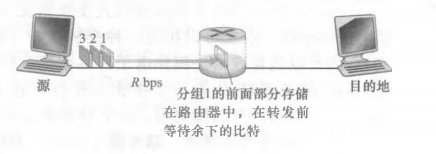
\includegraphics[width=0.6\textwidth]{image/chapter01/存储转发.png}
    \caption{存储转发传输}
\end{figure}

    在图1.6所示的特定时刻,源已经传输了分组1的一部分,分组1的前沿已经到达了路由器。因为该路由器应用了存储转发机 制,所以此时它还不能传输已经接收的比特,而是必须先缓存(即“存储”)该分组的比 特。仅当路由器已经接收完了该分组的所有比特后,它才能开始向出链路传输(即“转发”)该分组。

    对于一般情况(暂不考虑传播时延):\emph{通过由$N$条速率均为$R$的链路组成的路径(意味着在源和目的地中由$N - 1$台路由器),从源到目的地发送一个分组},我们看到的端对端时延是:

$$
    d_{端到端} = N\frac{L}{R}
$$

\subsubsection{排位延时和分组丢失}

    对于每条相连的链路,该分组交换机具有一个输出缓存(output buffer,也称为输出队列(output queue)),它用于存储路由器准备发往那条链路的分组。该输出缓存在分组交换中起着重要的作用。

    如果到达的分组需要传输到某条链路,但发现该链路正忙于传输其他分组,该到达分组必须在输出缓存中等待。因此,除了存储转发时延以外,分组还要承受输岀缓存的排队时延(queuing delay)。

    \emph{这些时延是变化的,变化的程度取决于网络的拥塞程度。}又因为缓存空间的大小是有限的,因此可能存在一个到达的分组但是缓存已经充满的情况,此时就将出现分组丢失(丢包, $packet loss$)。

\subsubsection{转发表和路由选择协议}

    路由器从与它相连的一条通信链路得到分组,然后向与它相连的另一条通信链路转发该分组。但是路由器怎样决定它应当向哪条链路进行转发呢?

    在因特网中,每个端系统具有一个称为IP地址的地址。当源主机要向目的端系统发 送一个分组时,源在该分组的首部包含了目的地的IP地址。当一个分组到达网络中的路由器时,路由器检查该分组的目的地址的 一部分,并向一台相邻路由器转发该分组。
    
    更特别的是,每台路由器具有一个转发表(forwarding table),用于将目的地址(或目的地址的一部分)映射成为输岀链路。当某分组到达一台路由器时,路由器检查该地址,并用这个目的地址搜索其转发表,以发现适当的出链路。路由器则将分组导向该出链路。

\subsubsection{电路交换}

    通过网络链路和交换机移动数据有两种基本方法:电路交换(circuit switching)和分组交换(packet switching)。

    在电路交换网络中,在端系统间通信会话期间,预留了端系统间沿路径通信所需要的资源(缓存,链路传输速率)。在分组交换中,这些资源则不会预留,但是得承担其不得不等待接入通信线路的代价。

    传统的电话网络是电路交换网络的例子。在发送方能够发送信息之前,该网络必须在发送方和接收方之间建立一条连接。这是一个名副其实的连接,因为此时沿着发送方和接收方之间路径上的交换机都将为该连接维护连接状态。
    
    用电话的术语来说,该连接被称为一条电路(circuit)。当网络创建这种电路时,它也在连接期间在该网络链路上预留了恒定的传输速率(表示为每条链路传输容量的一部分)。既然已经为该发送方-接收方连接预留了带宽,则发送方能够以确保的恒定速率向接收方传送数据。

\begin{figure}[!htbp]
    \centering
    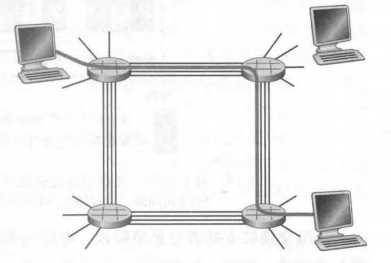
\includegraphics[width=0.6\textwidth]{image/chapter01/电路交换.png}
    \caption{简单电路交换网络}
\end{figure}

    如上图,在这个网络中,用四条链路互联了四台电路交换机。当两台主机要通信时,该网络在两台主机之间创建一条专用的端到端链接($end-to-end$)。因为每条链路具有四条电路,对于由端到端链接所使用的每条链路而言,该连接在连接期间获得链路总传输总量的1/4。

\paragraph{电路交换网络中的复用}

    链路中的电路是通过频分复用 (Frequency- Division Multiplexing, FDM )或时分复用(Time-Division Multiplexing, TDM)来实现的。

    对于FDM,链路的频谱由跨越链路创建的所有连接共享。特别是,在连接期间链路为每条连接专用一个频段。FDM通过将不同的信号调制到不同的频带上,然后将这些频带合并到一个复合信号中,实现了多路信号的同时传输。在FDM系统中,链路的频谱被划分为一系列不重叠的子带,每个子带用于传输一个独立的信号或连接。每个连接被分配一个特定的频带,该频带在整个连接的生命周期中都是专用的。

    由于每个连接在链路上使用独占的频段,因此不同连接之间的信号不会相互干扰。这使得多个连接可以同时在链路上传输,并且可以实现频谱的高效利用。
    
    需要注意的是,FDM是一种静态频分复用技术,即连接在建立时会占用固定的频段,并且在连接的整个生命周期内保持不变。由于频谱资源是有限的,所以在设计FDM系统时,需要合理划分频带以满足所有连接的需求,并确保频段之间的不重叠,以避免干扰和交叉干扰。
    
    对于于一条TDM链路,时间被划分为固定期间的帧,并且每个帧又被划分为固定数量的时隙。当网络跨越一条链路创建一条连接时,网络在每个帧中为该连接指定一个时隙。这些时隙专门由该连接单独使用,一个时隙(在每个帧内)可用于传输该连接的数据

\begin{figure}[!htbp]
    \centering
    \includegraphics[width=0.6\textwidth]{image/chapter01/FDM和TDM.png}
    \caption{FDM和TDM的不同演示}
\end{figure}

\paragraph{分组交换与电路交换的对比}

    分组交换的批评者经常争辩说,分组交换不适合实时服务(例如,电话和视频会议),因为它的端到端时延是可变的和不可预测的(主要是因为排队时延的变动和不可预测所致)。

    分组交换的支持者却争辩道:

\begin{itemize}
    \item [1)] 它提供了比电路交换更好的带宽共享
    \item [2)] 它比电路交换更简单、更有效,实现成本更低
\end{itemize}

    其实有一个例子能够很好的证明分组交换会更加有效,只要同时活跃的用户不够多的情况下,分组交换总是优于电路交换,因为分组交换没有静默期这一情况。\emph{分组交换差不多总是提供了与电路交换相同的性能,并且允许在用户数量是其3倍时情况也是如此}。

    电路交换不考虑需求,而预先分配了传输链路的使用,这使得已分配而并不需要的链路时间未被利用。另一方面,分组交换按需分配链路使用。链路传输能力将在所有需要在链路上传输分组的用户之间逐分组地被共享。

\subsubsection{网络的网络}

    端系统经过一个接入ISP与因特网相连,该ISP不必是电信局或电缆局,如何解决因特网中数以万计的用户通过接入ISP互联是一个很大的问题。而要解决这个难题,接入ISP自身必须互联。通过创建\emph{网络的网络}可以做到这一点。

\paragraph{网络结构1} 用单一的\emph{全球传输}ISP互联所有接入ISP。假想的全球传输ISP是一个由路由器和通信链路构成的网络,该网络不仅跨越全球,而且 至小具有一台路由器靠近数十万接入ISP中的每一个。

    为了有利可图,该全球ISP自然要向每一个接入ISP收费,故接入ISP被认为是客户(customer),而全球传输ISP被认为是提供商(provider)。

\paragraph{网络结构2} 由数十万接入ISP和多个全球传输ISP组成,现在能够根据价格和服务因素在多个竞争的全球传输提供商之间进行选择。

    网络结构2是一种两层的等级结构,其中全球传输提供商位于顶层,而接入ISP位于底层。这假设了全球传输ISP不仅能够接近每个接入ISP,而且发现经济上也希望这样做。但是,世界上是没有哪一个ISP是无处不在的。

\paragraph{网络结构3} 在任何给定的区域,可能有一个区域ISP(regional ISP),区域中的接入ISP与之连接。每个区域ISP则与第一层ISP(tier-1 ISP)连接。第一层ISP类似于我们假想的全球传输ISP,尽管它不是在世界上每个城市中都存在,但它确实存在。

    在这个等级结构的每一层,都有客户-提供商关系。值得注意的是,第一层1SP不向任何人付费,因为它们位于该等级结构的顶部。这个多层等级结构仍然仅仅是今天因特网的粗略近似。

\paragraph{网络结构4} 在等级化网络结构3上增加存在点(Point of Presence, PoP)、多宿、对等和因特网交换点。PoP存在于等级结构的所有层次,但底层(接入ISP)等级除外。一个POP只是提供商网络中的一台或多台路由器 (在相同位置)群组,其中客户ISP能够与提供商ISP连接。对于要与提供商PoP连接的客户网络,它能从第三方电信提供商租用高速链路将它的路由器之一直接连接到位于该PoP的一台路由器。

    客户ISP向它们的提供商ISP付费以获得全球因特网互联能力。客户ISP支付给提供商ISP的费用数额反映了它通过提供商交换的通信流量。为了减少这些费用,位于相同等级结构层次的邻近一对ISP能够对等(peer),也就是说,能够直接将它们的网络连到一起,使它们之间的所有流量经直接连接而不是通过上游的中间ISP传 输。当两个ISP对等时,通常不进行结算,即任一个ISP不向其对等付费。

    沿着这些相同路线,第三方公司能够创建一个因特网交换点(Internet Exchange Point, TXP),IXF是一个汇合点,多个ISP能够在这里一起对等。IXP通常位于一个有自己的交换机的独立建筑物中。

\paragraph{网络结构5} 下图中显示了网络结构5,它通过在网络结构4顶部增加内容提供商网络(content provider network )构建而成。

\begin{figure}[!htbp]
    \centering
    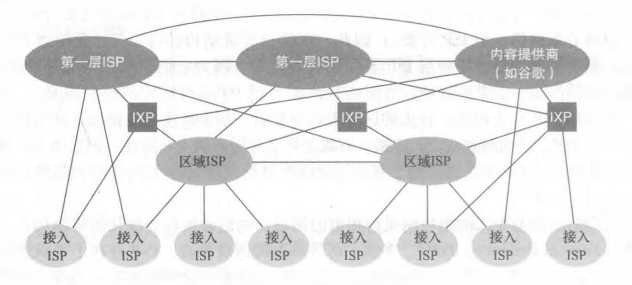
\includegraphics[width=0.6\textwidth]{image/chapter01/网络结构5.png}
    \caption{ISP的互联}
\end{figure}

    较低层的ISP与较高层的ISP相连,较高层ISP彼此互联。用户和内容提供商是较低层ISP的客户,较低层ISP是较高层ISP的客户。近年来,主要的内容提供商也已经创建自己的网络,直接在可能的地方与较低层ISP互联。

\section{分组交换网中的时延、丢包和吞吐量}

    在理想情况下,我们希望因特网服务能够在任意两个端系统之间随心所欲地瞬间移动数据而没有任何数据丢失。但是,显然是一个极其困难的目标,计算机网络\emph{必定要限制在端系统之间的吞吐量(每秒能够传送的数据量),在端系统之间引入时延,而且实际上也会丢失分组}。

\subsection{分组交换网中的时延概述}

    分组从一台主机(源)出发,通过一系列路由器传输,在另一台主机(目的地)中结束它的历程。该分组在沿途的每个节点经受了几种不同类型的时延。这些时延最为重要的是节点处理时延(nodal processing delay)、排队时延(queuing delay)、传输时延(transmission delay)和传播时延(propagation delay),这些时延总体累加起来是节点总时延(tolal nodal delay)。

\subsubsection{时延的类型}

    作为源和目的地之间的端到端路由的一部分,一个分组从上游节点通过路由器A向路由器B发送。

\begin{figure}[!htbp]
    \centering
    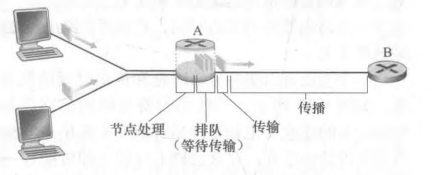
\includegraphics[width=0.6\textwidth]{image/chapter01/时延类型.png}
    \caption{路由器A上的节点时延}
\end{figure}

\begin{itemize}
    \item [1)] 处理时延
    \subitem 检查分组首部和决定将该分组导向何处所需要的时间是处理时延的一部分。 
    \item [2)] 排队时延
    \subitem 在队列中,当分组在链路上等待传输时,它经受排队时延。一个特定分组的排队时延长度将取决于先期到达的正在排队等待向链路传输的分组数量。如果该队列是空的,并且当前没有其他分组正在传输,则该分组的排队时延为0。
    \item [3)] 传输时延
    \subitem 假定分组以先到先服务方式传输——这在分组交换网中是常见的方式,仅当所有已经到达的分组被传输后,才能传输刚到达的分组。用L比特表示该分组的长度,用R bps(即b/s)表示从路由器A到路由器B的链路传输速率。传输时延是L/R。
    \item [4)] 传播时延
    \subitem 一旦一个比特被推向链路,该比特需要向路由器B传播。从该链路的起点到路由器B传播所需要的时间是传播时延。该比特以该链路的传播速率传播。该传播时延等于两台路由器之间的距离除以传播速率。即传播时延是其中d是路由器A和路由器B之间的距离,s是该链路的传播速率
    \item [5)] 传输时延与传播时延的比较
    \subitem 传输时延是路由器推出分组所需要的时间,它是分组长度和链路传输速率的函数,而与两台路由器之间的距离无关。
    \subitem 传播时延是一个比特从一台路由器传播到另一台路由器所需要的时间,它是两台路由器之间距离的函数,而与分组长度或链路传输速率无关。
    \subitem 我们可以用一个小例子来说明区别,假如有一个十辆车的车队,那么公路上行驶(即传播),而每隔100km就有一个收费站(路由器),而该车队必须整车队一起出发,因此收费站必须处理完十辆车后,车队开始出发。且无论该车队的第一辆汽车何时到达收费站,它在入口处等待,直到其他9辆汽车到达并整队依次前行。收费站将车队处理完之前(整个车队存储在收费站),因此收费站处理就相当于传输时延,而到达下一个收费站就相当于传播时延。
    \begin{figure}[!htbp]
        \centering
        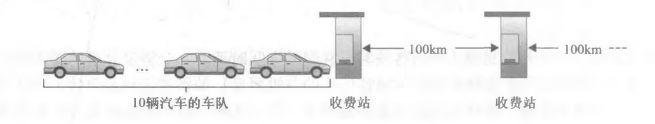
\includegraphics[width=0.6\textwidth]{image/chapter01/收费站类比.png}
        \caption{车队的类比}
    \end{figure}
\end{itemize}

    如果令$d_{proc},\ d_{queue},\ d_{trans},\ d_{prop}$分别表示处理时延、排队时延、传输时延和传播时延, 则节点的总时延由下式给定:

$$
    d_{total} = d_{proc} + d_{queue} + d_{trans} + d_{prop}
$$

    处理时延$d_{proc}$通常是微不足道的;然而,它对一台路由器的最大吞吐量有重要影响,最大吞吐量是一台路由器能够转发分组的最大速率。

\subsection{排队时延和丢包}

    节点时延的最为复杂和有趣的成分是排队时延$d_{queue}$。与其他三项时延($d_{proc},\ d_{trans},\ d_{prop}$)不同的是,排队时延对不同的分组可能是不同的。因此,当表征排队时延时,人们通常使用统计量来度量,如平均排队时延、 排队时延的方差和排队时延超过某些特定值的概率。

    什么时候排队时延大,什么时候又不大呢?该问题的答案很大程度\emph{取决于流量到达该队列的速率、链路的传输速率和到达流量的性质,即流量是周期性到达还是以突发形式到达}。

    我们假设令a表示分组到达队列的平均速率(a的单位是分组/秒,即pkt/s)。前面讲过R是传输速率,即从队列中推出比特的速率(以bps即b/s为单位)。为了简单起见,也假定所有分组都是由L比特组成的。则比特到达队列的平均速率是La bps。最后,假定该队列非常大,因此它基本能容纳无限数量的比特。比率La/R被称为流量强度(traffic intensity),它在估计排队时延的范围方面经常起着重要的作用。

    如果La/R>l,则比特到达队列的平均速率超过从该队列传输岀去的速率。因此:\emph{设计系统时流量强度不能大于1}。

    如果$La/R \le 1$,此时到达流量的性质影响排队时延。如果分组周期性到达,即每$L/R$秒到达一个分组,则每个分组将到达一个空队列,不会有排队时延;若以突发形式到达,则可能有很大的平均排队时延。

    通常,到达队列的过程是随机的,即到达并不遵循任何模式,分组之间的时间间隔是随机的。无论如何,随着流量强度接近1,平均排队长度变得越来越长。平均排队时延与流量强度的定性关系如下图所示。

\begin{figure}[!htbp]
    \centering
    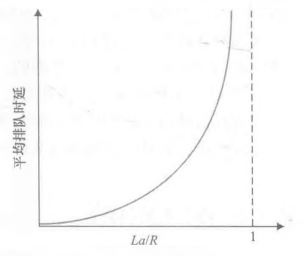
\includegraphics[width=0.4\textwidth]{image/chapter01/平均时延与流量强度的关系.png}
    \caption{平均排队时延与流量强度的关系}
\end{figure}

    \emph{随着流量强度接近于1,平均排队时延迅速增加。该强度的少量增加将导致时延大比例增加。}

\subsubsection{丢包}

    在现实中,一条链路前的队列只有有限的容量,尽管排队容量极大地依赖于路由器设计和成本。因为该排队容量是有限的,随着流量强度接近1,排队时延并不真正趋向无穷大。相反,到达的分组将发现一个满的队列。由于没有地方存储这个分组,路由器将丢弃(drop)该分组,即该分组将会丢失(lost)。

    分组丢失的比例随着流量强度增加而增加。因此,一个节点的性能常常不仅根据时延来度量,而且根据丢包的概率来度量。

\subsection{端到端时延}

    我们现在考虑从源到目的地的总时延。为了能够理解这个概念,假定在源主机和目的主机之间有N-1台路由器。我们还要假设该网络此时是无拥塞的(因此排队时延是微不足道的),在每台路由器 和源主机上的处理时延是dpw,每台路由器和源主机的输出速率是R bps,每条链路的传播时延是$d_{prop}$。节点时延累加起来,得到端到端时延:

$$
    d_{end-end} = N(d_{proc} + d_{trans} + d_{prop})
$$

\subsection{计算机网络中的吞吐量}

    假设我们从主机A到主机B跨越计算机网络传输一个大文件。在任何时间瞬间的瞬时吞吐量(instantaneous throughput)是主机B接收到该文件的速率(以bps计)。如果该文件由F比特组成,主机B接收到所有F比特用去T秒, 则文件传送的平均吞吐量(average throughput)是F/T bps。

    首先,我们考虑两个例子。令$R_{s}$表示服务器与路由器之间的链路速率;$R_{c}$表示路由器与客户之间的链路速率。假定在整个网络中只有从该服务器到客户的比特在传送。

    显然,这台服务器不能以快于$R_{s}$bps的速率通过其链路注入比特;这台路由器也不能以快于$R_{c}$bps的速率转发比特。如果$R_s < R_c$,则在给定的吞吐量$R_s$bps的情况下,由该服务器注入的比特将顺畅地通过路由器“流动”,并以速率$R_s$bps到达客户。 另一方面, 如果$R_c < R_s$,则该路由器将不能像接收速率那样快地转发比特。在这种情况下,比特将以速率$R_c$离开该路由器,从而得到端到端吞吐量$R_c$。

    因此, 对于这种简单的两链路网络,其吞吐量是$min\{R_c, R_s\}$ 这就是说,它是瓶颈链路(bottleneck link)的传输速率。因此,我们就近似的得到了传输一个F比特的大文件所需要的时间是$F/min\{R_c, R_s\}$。

\begin{figure}[!htbp]
    \centering
    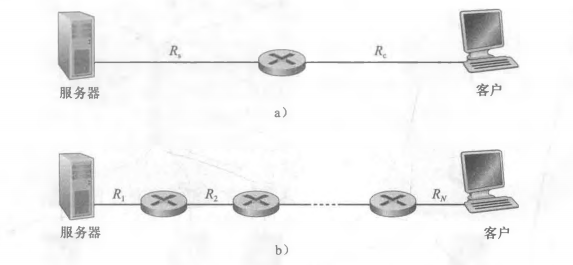
\includegraphics[width=0.6\textwidth]{image/chapter01/简单链路的吞吐量.png}
    \caption{一个文件从服务器传送到客户的吞吐量}
\end{figure}

    对于一个在服务器和客户之间具有N条链路的网络,我们发现从服务器到客户的文件传输吞吐量是$min\{R_1, R_2,..., R_N\}$,这同样仍是沿着服务器和客户之间路径的瓶颈链路的速率。

    吞吐量取决于数据流过的链路的传输速率。当没有其他干扰流量时,其吞吐量能够近似为沿着源和目的地之间路径的最小传输速率。 同时,吞吐量不仅取决于沿着路径的传输速率,而且取决于干扰流量。特别是,如果许多其他的数据流也通过这条链路流动,一条具有高传输速率的链路仍然可能成为文件传输的瓶颈链路。

\section{协议层次及其服务模型}

\subsection{分层的体系结构}

    利用分层的体系结构,我们可以讨论一个大而复杂系统的定义良好的特定部分。这种简化本身由于提供模块化而具有很高价值,这使某层所提供的服务实现易于改变。只要该层对其上面的层提供相同的服务,并且使用来自下面层次的相同服务,当某层的实现变化时,该系统的其余部分保持不变。

\subsubsection{协议分层}

    为了给网络协议的设计提供一个结构,网络设计者以分层(layer)的方式组织协议以及实现这些协议的网络硬件和软件。

    我们关注某层向它的上一层提供的服务(service),即所谓一层的服务模型(service model)。

    \emph{一个协议层能够用软件、硬件或者两者结合的方式来实现}。对于HTTP和SMTP这样的应用层协议总是在端系统中用软件实现,而物理层和数据链路层负责处理跨越特定链路的通信,因此在与给定链路相关联的网络接口卡中实现。网络层经常是硬件和软件实现的混合体。需要注意的是,\emph{一个第n层协议也分布在构成该网络的端系统、分组交换机和其他组件}。

    协议分层具有概念化和结构化的优点,这使得更新组件更为容易,但是,分层的一个潜在缺点是一层可能冗余较低层的功能。第二个潜在缺点是某层的功能可能需要仅在其他层才出现的信息,这又违反了层次分离的目标。

    各层的所有协议被称为协议栈(protocol stack)。因特网的协议栈由五个层次组成:物理层、链路层、网络层、运输层和应用层。

\begin{figure}[!htbp]
    \centering
    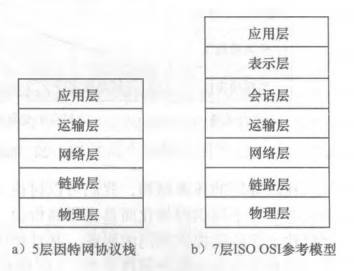
\includegraphics[width=0.6\textwidth]{image/chapter01/协议栈模型.png}
    \caption{因特网协议栈和OSI参考模型}
\end{figure}

\paragraph{应用层} 应用层是网络应用程序及它们的应用层协议存留的地方。

    应用层协议分布在多个端系统上,而一个端系统中的应用程序使用协议与另一个端系统中的应用程序交换信息分组。我们把这种位于应用层的信息分组称为报文(message)。

\paragraph{运输层} 因特网的运输层在应用程序端点之间传送应用层报文。

    在因特网中,有两种运输协议,即TCP和UDP,利用其中的任一个都能运输应用层报文。在本书中,我们把运输层的分组称为报文段。(segment)。

\paragraph{网络层}

    因特网的网络层负责将称为数据报(datagram)的网络层分组从一台主机移动到另一台主机。在一台源主机中的因特网运输层协议(TCP或UDP)向网络层递交运输层报文段和目的地址,就像你通过邮政服务寄信件时提供一个目的地址一样。

    因特网的网络层包括著名的网际协议IP,该协议定义了在数据报中的各个字段以及端系统和路由器如何作用于这些字段。IP仅有一个,所有具有网络层的因特网组件必须运行IP。因特网的网络层也包括决定路由的路由选择协议,它根据该路由将数据报从源传输到目的地。因特网具有许多路由选择协议。

    尽管网络层包括了网际协议和一些路由选择协议,但通常把它简单地称为IP层,这反映了IP是将因特网连接在一起的黏合剂这样的事实。

\paragraph{链路层}

    因特网的网络层通过源和目的地之间的一系列路由器路由数据报。为了将分组从一个节点(主机或路由器)移动到路径上的下一个节点,网络层必须依靠该链路层的服务。

    由链路层提供的服务取决于应用于该链路的特定链路层协议。因为数据报从源到目的地传送通常需要经过几条链路,一个数据报可能被沿途不同链路上的不同链路层协议处理。网络层将受到来自每个不同的链路层协议的不同服务。在本书中,我们把链路层分组称为帧(frame)。

\paragraph{物理层}

链路层的任务是将整个帧从一个网络元素移动到邻近的网络元素,而物理层的任务是将该帧中的一个个比特从一个节点移动到下一个节点。在这层中的协议仍然是链路相关的,并且进一步与该链路(例如,双绞铜线、单模光纤)的实际传输媒体相关。

\subsubsection{OSI模型}

    因特网协议栈不是唯一的协议栈,是在20世 纪70年代后期,国际标准化组织(ISO)提出计算机网络围绕7层来组织,称为开放系统互连(OSI)模型。

    OSI参考模型的7层是:应用层、表示层、会话层、运输层、网络层、数据链路层和物理层。这些层次中,5层的功能大致与它们名字类似的因特网对应层的功能相同。所以,我们来考虑0SI参考模型中附加的两个层,即表示层和会话层。表示层的作用是使通信的应用程序能够解释交换数据的含义。这些服务包括数据压缩和数据加密(它们是自解释的)以及数据描述(这使得应用程序不必担心在各台计算机中表示/存储的内部格式不同的问题)。会话层提供了数据交换的定界和同步功能,包括了建立检查点和恢复方案的方法。

\subsection{封装}

    下图显示了这样一条物理路径:数据从发送端系统的协议栈向下,沿着中间的链路层交换机和路由器的协议栈上上下下,然后向上到达接收端系统的协议栈。路由器和链路层交换机都是分组交换机。与端系统类似,路由器和链路层交换机以多层次的方式组织它们的网络硬件和软件。而路由器和链路层交换机并不实现协议栈中的所有层次。

    图中也说明了一个重要概念:封装(encapsulation)。在发送主机端,一个应用层报文(application-layer message)(图中的$M$)被传送给运输层。在最简单的情况下,运输层收取到报文并附上附加信息(所谓运输层首部信息,图中的$H_t$,该首部将被接收端的运输层使用。应用层报文和运输层首部信息一道构成了运输层报文段(transport layer segment)。
    
    运输层报文段因此封装了应用层报文。附加的信息也许包括了下列信息: 允许接收端运输层向上向适当的应用程序交付报文的信息;差错检测位信息,该信息让接收方能够判断报文中的比特是否在途中已被改变。
    
    运输层则向网络层传递该报文段,网络层增加了如源和目的端系统地址等网络层首部信息(图中的$H_n$,生成了网络层数据报(network-layer datagram)。该数据报接下来被传递给链路层,链路层(自然而然地)增加它自己的链路层首部信息并生成链路层帧(link layer frame)。
    
    所以我们看到,在每一层,一个分组具有两种类型的字段:首部字段和有效载荷字段(payload field)。有效载荷通常是来自上一层的分组。

\begin{figure}[!htbp]
    \centering
    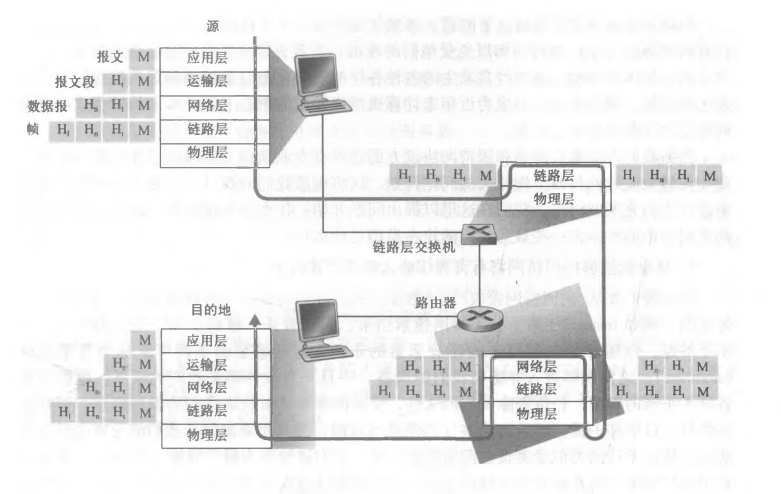
\includegraphics[width=0.6\textwidth]{image/chapter01/主机、路由器和链路交换层的传输.png}
    \caption{主机、路由器和链路交换机}
\end{figure}

\section{面对攻击的网络}

\subsection{通过因特网放入病毒}

    因为我们要从/向因特网接收/发送数据,所以我们将设备与因特网相连。不幸的是,伴随好的东西而来的还有恶意的东西,这些恶意的东西可统称为恶意软件(malware),它们能够进入并感染我们的设备。我们的受害主机也可能成为数以千计的类似受害设备网络中的一员,它们被统称为僵尸网络(botnet)。

    至今为止的多数恶意软件是自我复制(self-replicating)的:一旦它感染了一台主机, 就会从那台主机寻求进人因特网上的其他主机,从而形成新的感染主机,再寻求进入更多的主机。

    病毒(virus)是\emph{一种需要某种形式的用户交互来感染用户设备的恶意软件}。

    蠕虫(worm)是\emph{一种无须任何明显用户交互就能进入设备的恶意软件}。

\subsection{攻击服务器和网络基础设施}

    另一种宽泛类型的安全性威胁称为拒绝服务攻击(Denial-of Service (DoS) attack)。顾名思义,DoS攻击使得网络、主机或其他基础设施部分不能由合法用户使用。

    大多数因特网DoS攻击属于下列三种类型之一:

\begin{itemize}
    \item [1)] 弱点攻击。这涉及向一台目标主机上运行的易受攻击的应用程序或操作系统发送制作精细的报文。如果适当顺序的多个分组发送给一个易受攻击的应用程序或操作系统,该服务器可能停止运行,或者更糟糕的是主机可能崩溃。
    \item [2)] 带宽洪泛。攻击者向目标主机发送大量的分组,分组数量之多使得目标的接入链路变得拥塞,使得合法的分组无法到达服务器。
    \item [3)] 连接洪泛。攻击者在目标主机中创建大量的半开或全开TCP连接。该主机因这些伪造的连接而陷入困境,并停止接受合法的连接。
\end{itemize}

    下图中显示的分布式DoS ( Distributed DoS, DDoS)中,攻击者控制多个源并让每个源向目标猛烈发送流量。使用这种方法,遍及所有受控源的聚合流量速率需要大约R的能力来使该服务陷入瘫痪。DDoS攻击充分利用由数以千计的受害主机组成的僵尸网络,这在今天是屡见不鲜的。

\begin{figure}[!htbp]
    \centering
    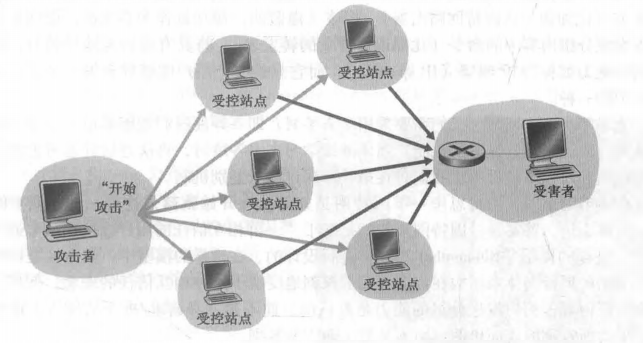
\includegraphics[width=0.6\textwidth]{image/chapter01/分布式拒绝服务攻击DDOS.png}
    \caption{分布式拒绝服务攻击}
\end{figure}

\subsection{嗅探分组}

    无所不在的因特网接入极为便利并让移动用户方便地使用令人惊奇的新应用程序的同时,也产生了严重的安全脆弱性一一在无线传输设备的附近放置一台被动的接收机,该接收机就能得到传输的每个分组的副本!这些分组包含了各种敏感信息,包括口令、社会保险号、商业秘密和隐秘的个人信息。记录每个流经的分组副本的被动接收机被称为分组嗅探器(packet sniffer)。

    嗅探器也能够部署在有线环境中。在有线的广播环境中,如在许多以太网LAN中,分组嗅探器能够获得经该LAN发送的所有分组。

    因为分组嗅探器是被动的,也就是说它们不向信道中注入分组,所以难以检测到它们。因此,当我们向无线信道发送分组时,我们必须接受这样的可能性,即某些坏家伙可能记录了我们的分组的副本。

\subsection{伪装}

    生成具有任意源地址、分组内容和目的地址的分组,然后将这个人工制作的分组传输到因特网中,因特网将忠实地将该分组转发到目的地,这一切都极为容易。将具有虚假源地址的分组注入因特网的能力被称为IP哄骗(IP spoofing),而它只是一个用户能够冒充另一个用户的许多方式中的一种。

    为了解决这个问题,我们需要采用端点鉴别,即一种使我们能够确信一个报文源自我们认为它应当来自的地方的机制。

    